% !TEX root = ../template.tex
\section{Случаи из практики}

\subsection{Пример картинки}

Рандомный граф (\vref{pic:graph}). 

Для насильной привязки к месту использовать опцию \textbf{[H]}. \cite{float}

\begin{figure}[H]
	\centering
	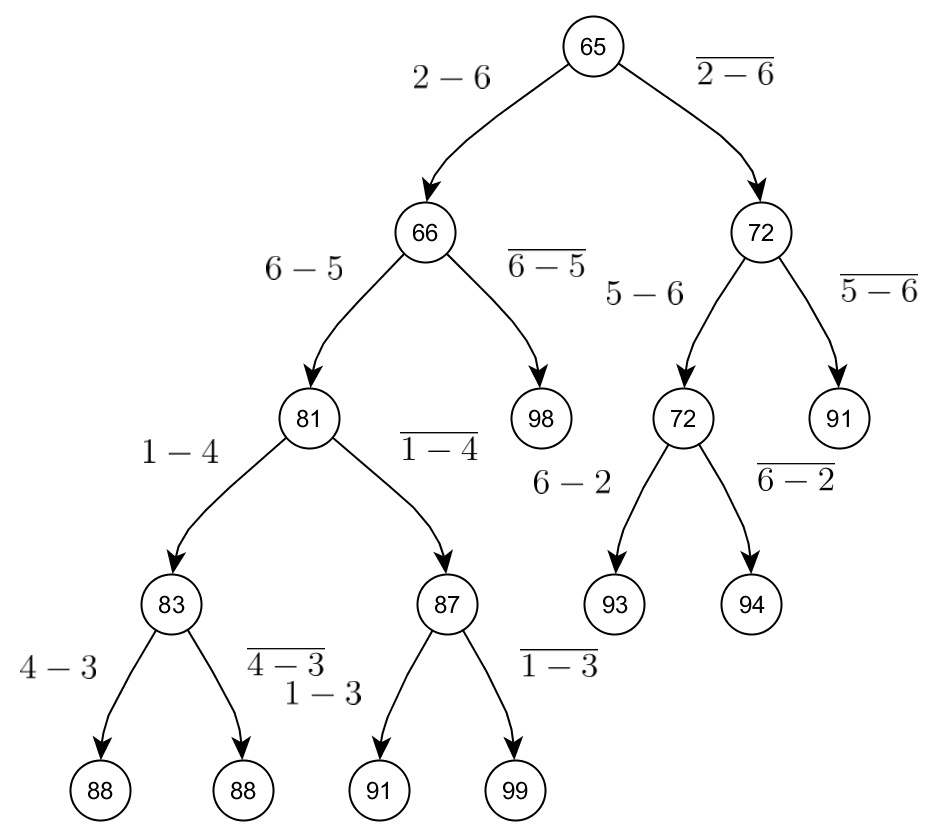
\includegraphics[width=0.56\textwidth]{full}
	\caption{Граф}
	\label{pic:graph}
\end{figure}

\subsection{Листинг с помощью \emph{listings}}

Пакет \emph{listings} имеет кучу мелких и не очень проблем, из-за которых пропадает желание его использовать.

Описание схемы на языке VHDL приведено в листинге~\ref{lst:VHDL}.
См.~\vref{app:matlab} для ещё одного примера.

\lstset{style=vhdl}
\begin{lstlisting}[label=lst:VHDL,caption=Описание схемы]
entity lab2 is
port(
	SW0,SW1,SW2,SW3,SW4 : in bit;
	LED0,LED1,LED2 : out bit;
	LED3,LED4,LED5 : out boolean
	);
end lab2;
architecture rtl of lab2 is
	signal TEMP : bit := '0';
begin
	LED2 <= '0';
	temp <= SW0 or SW1;
	LED1 <= TEMP and SW2;
	LED0 <= not TEMP;
	LED3 <= not(SW3 > SW4);
	LED4 <= not(SW3 = SW4);
	LED5 <= not(SW3 < SW4);
end rtl;
\end{lstlisting}

\subsection{Картинки с подкартинками}

Данные о максимальной частоте и минимальных временных задержках представлены на \vref{pic:base} (а так же \vref{pic:fmax} и \vref{pic:clk}). \cite{subcap}

\begin{figure}[H]
	\begin{subfigure}{.4\linewidth}
		\centering
		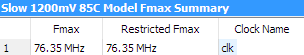
\includegraphics[width=1\textwidth]{fmax}
		\caption{Максимальная частота}
		\label{pic:fmax}
	\end{subfigure}
	\begin{subfigure}{.6\linewidth}
		\centering
		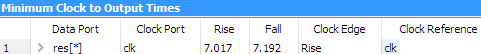
\includegraphics[width=1\textwidth]{clk}
		\caption{Минимальные задержки}
		\label{pic:clk}
	\end{subfigure}
\caption{Описание без оптимизации}
\label{pic:base}
\end{figure}

\subsection{Длинная подпись}

Результат моделирования синтезированной схемы представлен на \vref{pic:modeling}. 

\begin{figure}[H]
\centering
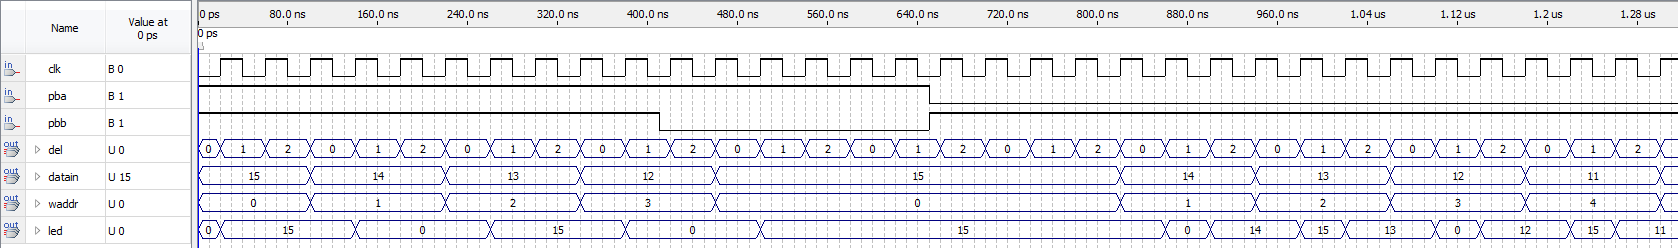
\includegraphics[width=1\textwidth]{modeling}
\caption{Результат моделирования схемы в редакторе диаграмм \\ (Коэффициент деления частоты = 3)}
\label{pic:modeling}
\end{figure}

Другой пример (см. \vref{tab:task}). 

Обратите внимание на расположение \string\caption\{\} снизу и при этом принудительное расположение подписи сверху с выравниванием вправо.

\begin{table}[H]
	\centering
	\begin{tabular}{|c|c|c|c|c|c|}
		\hline $\infty$ & $27$     & $13$     & $7$      & $45$     & $35$ 		\\
		\hline $21$     & $\infty$ & $14$     & $20$     & $19$     & $12$ 		\\
		\hline $10$     & $14$     & $\infty$ & $6$      & $32$     & $25$ 		\\
		\hline $7$      & $18$     & $5$      & $\infty$ & $38$     & $28$ 		\\
		\hline $32$     & $16$     & $23$     & $27$     & $\infty$ & $23$ 		\\
		\hline $30$     & $10$     & $24$     & $28$     & $18$     & $\infty$	\\
		\hline		
	\end{tabular}
	\caption{Заданная матрица \\ задачи дискретного программирования}
	\label{tab:task}
\end{table}

\subsection{Русские буквы в формулах}

Пока только такой вариант \vref{equ:rus} (можно использовать просто \string\text\{\}).

\begin{equation}
	\sum_{\textup{Какая-то лажа}}^{\textit{Какой-то курсив}} \textbf{Какой-то жирнич}
	\label{equ:rus}
\end{equation}

\subsection{Отрицание-подчёркивание в мат. режиме}

Просто $\overline{\textup{над}}~\underline{\textup{под}}$

Ещё пример:

\centerline{
	\large$y = \overline{
		\overline{
			\overline x_{3}x_{4}\overline{
				\overline{
					\overline x_{1}\overline x_{2}
				}
				\overline x_{5}
			}
		}
		~\overline{
			x_{2}\overline{
				\overline x_{1}\overline{
					x_{4}x_{5}
				}
			}
		}
		~\overline{
			x_{3}\overline{
				\overline{
					\overline x_{1}\overline x_{4}
				}
				\,\overline{
					\overline x_{2}\overline x_{5}
				}
			}
		}
	}
	$} \normalsize 

\subsection{No line here to end при использовании \textbackslash\textbackslash}

Два способа решения: создать минимальное пространство с помощью $\sim$\textbackslash\textbackslash, или использовать \string\vspace\{X pt\}.

\subsection{Таблица с картинкой}

Пример в \vref{tab:rs-map}.

\begin{table}[ht]
	\centering
	\begin{tabular}{|M{1cm}|M{8cm}|M{5cm}|}
		\hline Имя & Функциональный преобразователь & Логическое выражение выходов \\
		\hline inst & \raisebox{-0.85\totalheight}{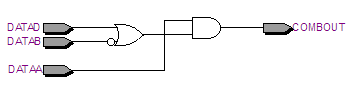
\includegraphics[width=0.45\textwidth]{rs-inst}} & $\overline{(Q'+\overline{R})\cdot S}\rightarrow Q$ \\
		\hline inst1 & \raisebox{-0.85\totalheight}{
\includegraphics[width=0.45\textwidth]{rs-inst1}} &  $\overline{\overline{Q''} \cdot R}\rightarrow \overline{Q}$ \\ \hline
	\end{tabular}
	\caption{Логические выражения для выходов RS-триггера}
	\label{tab:rs-map}
\end{table}

\subsection{Таблица с склееными и битыми ячейками}

Пример в \vref{tab:energy}.

Для склеивания строк требуется пакет \emph{multirow}. \cite{multirow}

\begin{table}[H]
	\centering
	\begin{tabular}{|c||*{4}{c|}}
		\hline \multirow{2}*{\textnumero} & \multirow{2}*{Частота, МГц} & \multirow{2}*{Период, нс} & \multicolumn{2}{c|}{Энергопотребление, мВт}\\
		\cline{4-2}\cline{5-2} &     &       & Полное & Динамическое	\\
		\hline 1               & 1   & 1000  & 64.79  & 0.05			\\
		\hline 2               & 10  & 100   & 65.45  & 0.51			\\
		\hline 3               & 50  & 20    & 68.38  & 2.53			\\
		\hline 4               & 100 & 10    & 72.05  & 5.06			\\
		\hline 5               & 150 & 6.667 & 75.71  & 7.59			\\ \hline
	\end{tabular}
	\caption{Зависимость энергопотребления от частоты}
	\label{tab:energy}
\end{table}

\subsection{Графики с TikZ/PGF}

Очень сложный метод, надо очень хорошо знать, что делаешь, иначе можно потратить день и не добиться результата. Зато в итоге можно получить качественное векторное изображение. В документации \emph{1200} страниц!!! \cite{pgf}

Пример на \vref{gr:energy}.

\begin{figure}[H]
	\begin{subfigure}{.5\linewidth}
		\centering
		\begin{tikzpicture}
			\begin{axis}[
				grid = both,
				axis line style = very thick,
				axis x line=bottom,
				axis y line=left,
				xlabel = {$f$, МГц},
    			ylabel = {$W$, мВт},
    			minor tick num = 1]
			\addplot coordinates {
    			(1,0.05) (10,0.51) (50,2.53) (100,5.06) (150,7.59) (200,10.13) (250,12.66)
			};
			\end{axis}
		\end{tikzpicture}
		\caption{Динамическое}
		\label{gr:din}
	\end{subfigure}
	\begin{subfigure}{.5\linewidth}
		\centering
		\begin{tikzpicture}
			\begin{axis}[
				grid = both,
				axis line style = very thick,
				axis x line=bottom,
				axis y line=left,
				xlabel = {$f$, МГц},
		  		ylabel = {$W$, мВт},
    			minor tick num = 1]
			\addplot coordinates {
    			(1,64.79) (10,65.45) (50,68.38) (100,72.05) (150,75.71) (200,79.38) (250,83.05)
			};
			\end{axis}
		\end{tikzpicture}
		\caption{Полное}
		\label{gr:stat}
	\end{subfigure}
\caption{Зависимость энергопотребления от частоты}
\label{gr:energy}
\end{figure}

\subsection{Надписи на стрелках}

Использует пакет \emph{mathtools}. \cite{mathtools}

\begin{table}[h!t]
	\centering
	\begin{tabular}{|c|cc|c|}
		\hline       & $x_3$        & $x_2$   & $B$ 			\\
		\hline $x_1$ & $-1$         & $-0.3$  & $10.2$ 			\\
			   $x_4$ & $-1$         & $-0.7$  & $11.4$ 			\\
		\hline $x_5$ & \textbf{2.5} & $-0.25$ & \textbf{-10.5}	\\
		\hline $f$   & \textbf{-1}  & $-2.3$  & $10.2$ 			\\ \hline
	\end{tabular}
	$\xRightarrow[\text{делим на 2.5}]{\text{преобразуем и}}$
	\begin{tabular}{|c|cc|c|}
		\hline       & $x_5$  & $x_2$  & $B$	\\
		\hline $x_1$ & $-0.4$ & $-0.4$ & $6$	\\
			   $x_4$ & $-0.4$ & $-0.8$ & $7.2$	\\
			   $x_3$ & $0.4$  & $0.1$  & $4.2$	\\
		\hline $f$   & $-0.4$ & $-2.4$ & $6$ 	\\ \hline
	\end{tabular}
\end{table}

\subsection{Случай с матрицей, где проверялся знак}

Текущие матрицы $P=\begin{bmatrix}
0 & 1 \\ 1 & -1
\end{bmatrix}$, $C^B=\begin{bmatrix}
0 & 1
\end{bmatrix}$

Допустимость: $X^B=P^{-1}B=\begin{bmatrix}
11.4 \\ 10.2
\end{bmatrix}\begin{matrix}
>0 \\ >0
\end{matrix}$ -- \textbf{допустимый}

\subsection{Скобочка}

\begin{equation}
	\left\{\begin{aligned}
		\max\left(x_1-2x_2\right), \\
		x_1+0.3x_2\leq 10.2, \\
		-x_1+0.4x_2\leq 1.2, \\
		x_1\geq 0, \\
		x_2\geq 0; \\
	\end{aligned}\right. \Longleftrightarrow
	\left\{\begin{aligned}
		\max\left(x_1-2x_2\right), \\
		x_1+0.3x_2+x_3=10.2, \\
		-x_1+0.4x_2+x_4=1.2, \\
		x_1\geq 0, \\
		x_2\geq 0; \\
		x_3\geq 0, \\
		x_4\geq 0; \\
	\end{aligned}\right.
\end{equation}

\subsection{Выравнивание в выражениях}

Выравнивание контролируется символом \&. \\

Условия Куна-Такера:
\begin{equation}
	\left\{\begin{aligned}
		&\nabla f(X^*)+\sum_{j=1}^{J} u_j \nabla g_j(X^*)=0,\\
		&u_j g_j(X^*)=0,~ j=1..J,\\
		&u_j \leq 0,~ j=1..J;\\
	\end{aligned}\right.
	\label{equ:kung}
\end{equation}

Подставим в формулу \vref{equ:kung}:

\begin{equation}
	\left\{\begin{aligned}
		-62x_1+4x_2+286+7u_1+10u_2-u_3=0,\\
		-68x_2+4x_1+388+12u_1+8u_2-u_4=0,\\
		u_1(7x_1+12x_2-84)=0,\\
		u_2(10x_1+8x_2-80)=0,\\
		u_3(-x_1)=0,\\
		u_4(-x_2)=0,\\
		u_1\leq 0,\\
		u_2\leq 0,\\
		u_3\leq 0,\\
		u_4\leq 0;\\
	\end{aligned}\right.
\end{equation}

\subsection{Графы}

Безумно неудобно и не стоит затраченных усилий. Лучше, быстрее и выгоднее воспользоваться \emph{yEd} или что-нибудь в таком духе и вставить картинку. Есть способ делать удобнее с Lua\TeX, но Lua\TeX~до сих пор не имеет официального релиза, поэтому пока не рекомендую. \\

Наибольший путь $1-2-4-5-6-7-8$ с весом $39$ представлен на \vref{pic:graph_max}.

\begin{figure}[H]
	\centering
	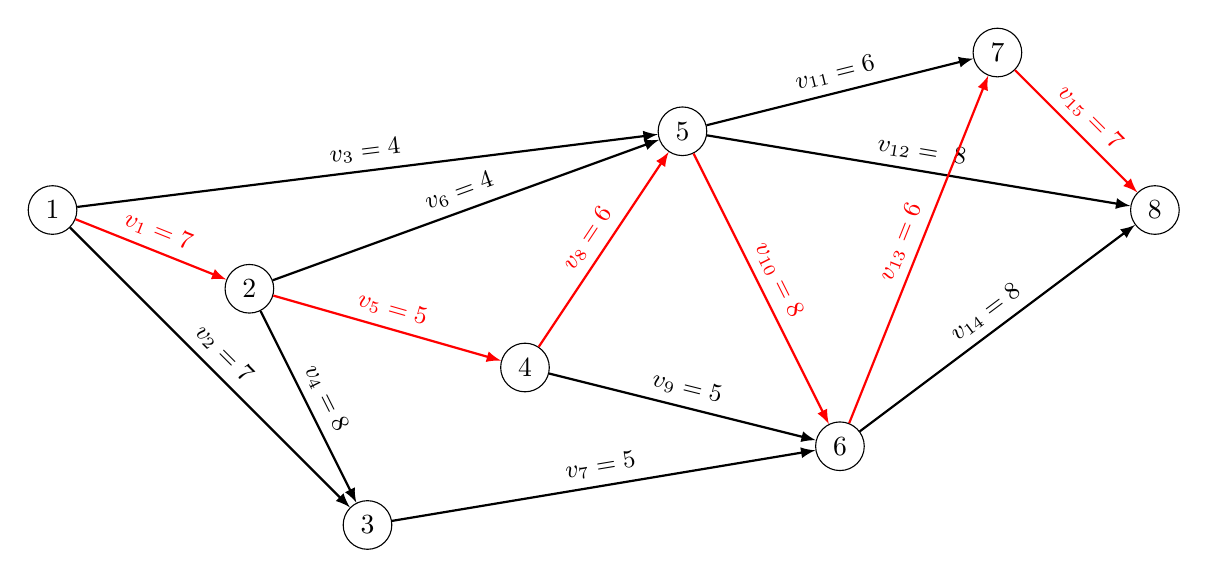
\begin{tikzpicture}[scale = 2]
		\node [circle,draw] (l1) at (0,2) {1};
		\node [circle,draw] (l2) at (1.25,1.5) {2};
		\node [circle,draw] (l3) at (2,0) {3};
		\node [circle,draw] (l4) at (3,1) {4};
		\node [circle,draw] (l5) at (4,2.5) {5};
		\node [circle,draw] (l6) at (5,0.5) {6};
		\node [circle,draw] (l7) at (6,3) {7};
		\node [circle,draw] (l8) at (7,2) {8};
		\path[->, thick, >=latex]
					(l1) edge[red] node[sloped, above]{\small $v_1=7$} (l2)
					(l1) edge node[sloped, above]{\small $v_2=7$} (l3)
					(l1) edge node[sloped, above]{\small $v_3=4$} (l5)
					(l2) edge node[sloped, above]{\small $v_6=4$} (l5)
					(l2) edge[red] node[sloped, above]{\small $v_5=5$} (l4)
					(l2) edge node[sloped, above]{\small $v_4=8$} (l3)
					(l3) edge node[sloped, above]{\small $v_7=5$} (l6)
					(l4) edge[red] node[sloped, above]{\small $v_8=6$} (l5)
					(l4) edge node[sloped, above]{\small $v_9=5$} (l6)
					(l5) edge[red] node[sloped, above]{\small $v_{10}=8$} (l6)
					(l5) edge node[sloped, above]{\small $v_{11}=6$} (l7)
					(l5) edge node[sloped, above]{\small $v_{12}=~8$} (l8)
					(l6) edge[red] node[sloped, above]{\small $v_{13}=6$} (l7)
					(l6) edge node[sloped, above]{\small $v_{14}=8$} (l8)
					(l7) edge[red] node[sloped, above]{\small $v_{15}=7$} (l8);
	\end{tikzpicture}
\caption{Наибольший путь}
\label{pic:graph_max}
\end{figure}

\subsection{Зачеркивания}

Пример: \\

$\begin{aligned}
	&2-6, 6-5, 1-4, 4-3 \Rightarrow \xcancel{6-2}, \xcancel{5-6}, \xcancel{5-2}, \xcancel{4-1}, \xcancel{4-2}, \xcancel{3-4}, \xcancel{3-1} \\
	&G_{2-6;6-5;1-4}=G_{2-6;6-5;1-4;4-3}\cup G_{2-6;6-5;1-4;\overline{4-3}} \\
\end{aligned}$ \\

Нельзя использовать зачёркивания пакета \emph{cancel} \cite{cancel} с самого первого слова: \\

\mbox{}\bcancel{Ещё} \cancel{такие} \st{вот} \cite{soul} \xcancel{иногда} $\cancelto{\textup{варианты}}{\textup{есть}}$.

\subsection{Внешние гиперссылки}

\url{www.fighting.ru}

\href{www.vk.com}{ВКонтакте}

\subsection{Некоторые символы в русском языке}

Дефис -

Тире ---

Такое тире -- не используется.

Тире "--- это модно.

"--* Прямая речь
<<Елочки и "`лапки"'>>

\subsection{Сборка \emph{varioref}$+$\emph{hyperref}$+$\emph{cleveref}$+$\emph{autonum}}

Весьма интересный и крайне нестабильный паровоз. Здесь распишу свои мысли по поводу использования этой гармошки. ~\\

Лучше всего определять эти пакеты в преамбуле друг за другом и в особом порядке: \emph{varioref}$\rightarrow$\emph{hyperref}$\rightarrow$\emph{cleveref}$\rightarrow$\emph{autonum}. Нарушение этого порядка ведёт к \emph{\textbf{огромной}} куче проблем. При этом пакет \emph{autonum} использует какой-то полумертвый пакет, из-за которого вылетает ошибка, в данном шаблоне это исправлено. ~\\

Пакет \emph{varioref} изменяет стиль ссылок, вводя новую команду \string\vref\{\}. \cite{varioref} Соль в том, что пакет определяет, где находится страница, на которую идет ссылка, и если она находится недалеко (следующая), то вместо номера он так и пишет "`на следующей странице"'. Также пакет не отображает страницу, если ссылка ведет на ту же страницу, где она и находится. То есть, данный пакет "--- это совмещение 
"`\string\ref\{\} на с. \string\pageref\{\}"' с немного расширенным функционалом. ~\\

Пакет \emph{hyperref} в эту сборку затесался из-за проблем совместимости, так что пропускаем. \cite{hyperref} ~\\

Пакет \emph{cleveref} изменяет стиль ссылок, вводя новые команды \string\cref\{\} и \\ \string\Cref\{\}. \cite{cleveref} Пакет определяет тип ссылки, и самостоятельно подписывает ее (например "`рис. \string\ref\{\}"' без необходимости писать "`рис."' самому). Встраивается в \emph{varioref}.

Важно знать одну вещь об этом пакете. В версии, находящейся в CTAN, и, соответственно, в сборке MiKTeX, существует баг, который нарушает основную особенность работы \emph{varioref} --- работает только ссылка вида "`на следующей странице"', и не работают все остальные виды ссылок. На \href{http://www.dr-qubit.org/latex.php#cleveref-docs}{сайте} автора пакета есть новая альфа-версия (ее не обновляли уже год), которая чинит баг, и она лежит в папке шаблона, чтобы не возиться с импортом.~\\

Пакет \emph{autonum} меняет работу с формулами. \cite{autonum} Например, он удаляет окружение \string\begin\{equation*\} и делает команду \string\[\string\] идентичной окружению \string\begin\{equation\}. При этом номера показываются только у тех формул, на которые присутствует ссылка, что немного упрощает работу.

\subparagraph{Как использовать?}

Использовать \string\vref\{\} для \emph{почти} всех случаев, где вам нужна ссылка на номер объекта с указанием страницы в сокращенном варианте ("`рис."') или \string\Vref\{\} для использования в начале предложения ("`Рисунок"'). При этом \emph{cleveref} встраивается в эту команду и будет подставлять тип ссылки автоматически. Из этого правила есть несколько исключений:

\begin{enumerate}
	\item Вам не нужна ссылка на страницу.

	Тогда используйте \string\cref\{\} и \string\Cref\{\}. Тип ссылки подставляется автоматически.
	\item Вы ссылаетесь на формулу.

	Используйте \string\cref\{\} и \string\Cref\{\} (\string\vref\{\} не~справляется), либо обычный \string\ref\{\} и/или \string\pageref\{\}. Автоматически тип подставляться не будет (т.~к. надпись "`ф-л."' или как-то так мне показалась крайне идиотской, а переопределить со склонениями нормально не получилось). Можно использовать связку \string\cref\{\} \string\vpageref\{\}, но результат не идеальный.

	\textbf{UPD.} В процессе работы над шаблоном команды \string\vref\{\} и \string\Vref\{\} переопределены, и весь этот пункт стал неактуальным.
	\item Вы ссылаетесь на листинг.

	Используйте обычный \string\ref\{\} и/или \string\pageref\{\} (проблемы те же, что и в пункте выше).
\end{enumerate}

Если вы хотите более подробно разобраться в работе этой сборки, поглядите документации.

\subsection{Очень длинные таблицы} \label{subsec:long}
Пример нагло украден с курса "`Документы и презентации в \LaTeX"' Д. Федоровых.

\begin{longtable}{|c|c|c|c|}
	\caption{Заголовок большой таблицы}
	\label{tab:longtable}\\
	\hline
	\textbf{RND1} & \textbf{RND2} & \textbf{RND3} & \textbf{RND4} \\ \hline
	\endfirsthead

	\captioncont
	\hline
	RND1 & RND2 & RND3 & RND4 \\ \hline
	\endhead

	\hline
	% \multicolumn{4}{r}{продолжение следует\ldots} \
	\endfoot

	\hline
	\endlastfoot

0,576745371 & 0,435853468 & 0,36384912  & 0,299047979 \\
0,064795364 & 0,028454613 & 0,751312059 & 0,693972684 \\
0,263563971 & 0,367508634 & 0,075536384 & 0,337780707 \\
0,957583964 & 0,431948588 & 0,938522377 & 0,464307785 \\
0,815740484 & 0,123129806 & 0,883432767 & 0,760983283 \\
0,445062335 & 0,157424268 & 0,883442259 & 0,300596338 \\
0,187159669 & 0,728663343 & 0,637199982 & 0,765684528 \\
0,41009848  & 0,457031472 & 0,142858106 & 0,602946607 \\
0,43315663  & 0,26058316  & 0,611667007 & 0,400328185 \\
0,824086963 & 0,27304335  & 0,244565296 & 0,219675484 \\
0,109578811 & 0,278478018 & 0,242519359 & 0,414669471 \\
0,62638369  & 0,737702261 & 0,696351048 & 0,256427487 \\
0,69779066  & 0,019424915 & 0,657473072 & 0,783698296 \\
0,14204222  & 0,817006985 & 0,669234791 & 0,728306309 \\
0,38941124  & 0,807135743 & 0,702842593 & 0,382494957 \\
0,203543688 & 0,969191131 & 0,822881425 & 0,212473701 \\
0,815740484 & 0,123129806 & 0,883432767 & 0,760983283 \\
0,445062335 & 0,157424268 & 0,883442259 & 0,300596338 \\
0,187159669 & 0,728663343 & 0,637199982 & 0,765684528 \\
0,41009848  & 0,457031472 & 0,142858106 & 0,602946607 \\
0,43315663  & 0,26058316  & 0,611667007 & 0,400328185 \\
0,824086963 & 0,27304335  & 0,244565296 & 0,219675484 \\
0,109578811 & 0,278478018 & 0,242519359 & 0,414669471 \\
0,62638369  & 0,737702261 & 0,696351048 & 0,256427487 \\
0,203543688 & 0,969191131 & 0,822881425 & 0,212473701 \\
0,826623142 & 0,181291269 & 0,054701556 & 0,386442059 \\
0,541365118 & 0,573617788 & 0,650112336 & 0,930417614 \\
0,957583964 & 0,431948588 & 0,938522377 & 0,464307785 \\
0,815740484 & 0,123129806 & 0,883432767 & 0,760983283 \\
0,445062335 & 0,157424268 & 0,883442259 & 0,300596338 \\
0,187159669 & 0,728663343 & 0,637199982 & 0,765684528 \\
\end{longtable}

\subsection{Обтекаемые рисунки/таблицы}
Также украдено с курса, упомянутого в \vref{subsec:long}. ~\\

\begin{wrapfigure}{l}{0.5\linewidth}
	
\includegraphics[width=\linewidth]{rs-inst1}
	\caption{Картинка с обтеканием}
\end{wrapfigure}
Прежде, чем анализировать "`что делать в сложной ситуации"', я думаю "`что можно сделать до того, как я попал в сложную ситуацию"'. 

Как сказано ранее, "`к поражению приводят множество факторов во время матча"'. Даже если вы исправили одну из проблем, иногда вы будете продолжать проигрывать по другим причинам.

\begin{wraptable}{r}{0.5\linewidth}
	\centering
	\begin{tabular}{|c|c|c|c|c|c|}
		\hline
		Год  & $P_x$ & $Q_x$ & $P_y$ & $Q_y$ & $n$  \\ \hline
		2008 &       & 36    &       & 32    & — 	\\ \hline
		2009 & 30    & 30    & 22    & 50    & 25\% \\ \hline
		2010 & 36    & 30    & 22    &       & 20\% \\ \hline
		2011 & 33    & 40    & 24    & 45    & 		\\ \hline
	\end{tabular}
	\caption{Обтекаемая таблица}
\end{wraptable}
Победа "--- это прекрасно, но даже если вы снова проигрываете, лучше всего сказать себе
"`Я могу сделать что-то, чего не мог раньше"' и ценить свой собственный прогресс.
Я думаю, что мышление "`Я тренируюсь, но у меня нет ощущения, что я играю лучше"' происходит из-за нарушения основной мотивации "`веселья"', "`фана"'. Так что, вне зависимости от исхода боя, очень важно позитивно смотреть на свои улучшения в игре.

Если вы устраните причины поражения одну за одной, даже если результат не наступит мгновенно, в будущем ваш винрейт стабилизируется и вы будете более уверены в своих решениях, расширите свои знания и кругозор в игре.

Вне зависимости от того, сколько вы исправите, если вы играете с другими игроками, иметь винрейт 100\% невозможно.

\subsection{Создание списка литературы}

Для этого можно использовать \emph{BiBLaTeX+Biber}.\cite{biblatex}

Создаёт и нумерует ссылки в порядке их упоминания.\cite{modelcheck} Стиль по ГОСТу (\emph{gost-numeric} в данном шаблоне) и его использование можно прочитать в описании стиля.\cite{gost}